\documentclass[10pt]{article}

\usepackage[margin=0.75in]{geometry}
\usepackage{amsmath,amsthm,amssymb}
\usepackage{xcolor}
\usepackage{cancel}
\usepackage{graphicx}
\usepackage{changepage}
\usepackage{circuitikz}
\usepackage{pgfplots}
\usepackage{physics}
\usepackage{hyperref}
\usepackage{siunitx}
\usepackage[breakable]{tcolorbox}
\usepackage[inline]{enumitem}

\theoremstyle{definition}
\newtheorem{problem}{Problem}
\newtheorem{soln}{Solution}

\pgfplotsset{compat=newest}
\usetikzlibrary{lindenmayersystems}
\usetikzlibrary{arrows}

\definecolor{incolor}{HTML}{303F9F}
\definecolor{outcolor}{HTML}{D84315}
\definecolor{cellborder}{HTML}{CFCFCF}
\definecolor{cellbackground}{HTML}{F7F7F7}
\newcommand{\eq}{=}
\usetikzlibrary{positioning, fit, calc}
\pgfdeclarelayer{background}  
\pgfsetlayers{background,main}

\makeatletter
\newcommand{\boxspacing}{\kern\kvtcb@left@rule\kern\kvtcb@boxsep}
\makeatother
\newcommand{\prompt}[4]{
    \ttfamily\llap{{\color{#2}[#3]:\hspace{3pt}#4}}\vspace{-\baselineskip}
}

\newcommand{\thevenin}[2]{
  \begin{center}
    \begin{circuitikz} \draw
      (0,0) -- (2,0) to[battery1, l_=$V_{Th}\eq#1$] (2,2) 
      to[resistor, l_=$R_{Th}\eq#2$] (0,2)
      ;
      \draw [o-] (-.07,2.079);
      \draw [o-] (-.07,0.079);
    \end{circuitikz}
  \end{center}
}

\newcommand{\norton}[2]{
  \begin{center}
    \begin{circuitikz} \draw
      (0,0) -- (3,0) to[american current source, l_=$I_{N}\eq#1$] (3,2) -- (0,2) (2,0)
      to[resistor, l=$R_{N}\eq#2$] (2,2)
      ;
      \draw [o-] (-.07,2.079);
      \draw [o-] (-.07,0.079);
    \end{circuitikz}
  \end{center}
}

\newcommand{\highlight}[1]{\colorbox{yellow}{$\displaystyle #1$}}

\hypersetup{
    colorlinks=true,
    linkcolor=blue,
    filecolor=magenta,      
    urlcolor=cyan,
    pdftitle={Overleaf Example},
    pdfpagemode=FullScreen,
    }

\NewDocumentCommand{\evalat}{sO{\big}mm}{%
  \IfBooleanTF{#1}
   {\mleft. #3 \mright|_{#4}}
   {#3#2|_{#4}}%
}

\title{Physics 2250: Problem Set VI}
\author{Jeremy Favro}
\date{\today}

\begin{document}

\maketitle

% PROBLEM 1
\begin{problem}
Consider the two pnp BJT's shown in the diagrams below. What regimes are each of the transistors operating in?
\begin{center} 
  \begin{circuitikz}
    
    \draw   \pgfextra{\ctikzset{bipoles/resistor/width=.4,
    bipoles/resistor/height=.2}} (0,0) coordinate(G) |- (2,4) to[battery1, l=$15\unit{\volt}$, invert] ++(0,-1) to[resistor, l=$10\unit{\kilo\ohm}$] ++(0,-0.75)
    node[pnp, anchor=C, yscale=-1, scale=0.85, tr circle](T){}
    (T.base) to[resistor, l_=$10\unit{\kilo\ohm}$] ++(-0.75,0) coordinate(R) to[battery1, l=$10\unit{\volt}$] (G -| R)
    (T.emitter) to[resistor, l=$1\unit{\kilo\ohm}$] (G -| T.emitter) node[ground]{} -- (G)
    ;

    \draw   \pgfextra{\ctikzset{bipoles/resistor/width=.4,
    bipoles/resistor/height=.2}} (4,0) coordinate(G) |- (6,4) to[battery1, l=$5\unit{\volt}$, invert] ++(0,-1) to[resistor, l=$10\unit{\kilo\ohm}$] ++(0,-0.75)
    node[pnp, anchor=C, yscale=-1, scale=0.85, tr circle](T){}
    (T.base) to[resistor, l_=$10\unit{\kilo\ohm}$] ++(-0.75,0) coordinate(R) -- (G -| R)
    (T.emitter) to[battery1, l=$13\unit{\volt}$] (G -| T.emitter) node[ground]{} -- (G)
    ;
  \end{circuitikz}
\end{center}
\end{problem}
\begin{soln}I'm not sure if this actually makes any sense but for the first circuit because $R_b=R_c$ but $V_{sb}<V_{sc}$ (the battery voltages) $V_b<V_c$.
  Then because $V_be=0.7\unit{\volt}$, $V_e<V_b$ so $V_e<V_b<V_c$ so, because this is a pnp transistor and not npn, the transistor is operating in the reverse active regime.
  \\
  Then for the second circuit because the base is at $0\unit{\volt}$ and $V_c<V_e$, $V_b<V_e>V_c$ which indicates that the transistor is operating in the saturated regime.

\end{soln}

% PROBLEM 2
\begin{problem}
  An Si BJT is set up in the ``common emitter'' configuration with the collector powered by $V_C=20\unit{\volt}$ across a load resistor of $R_L=500\unit{\ohm}$. The base is
  simply being supplied by $I_b$
  \end{problem}
  \begin{soln}~\\
    a)
    \begin{center} 
      \begin{circuitikz}
        \draw \pgfextra{\ctikzset{bipoles/resistor/width=.4,
        bipoles/resistor/height=.2}} 
        
        (0,0) node[ground]{} coordinate(G) node[npn, anchor=E, tr circle](T){}
        (T.base) to[american current source, l=$I_b$, invert] ++(-1.25,0)
        (T.collector) to[resistor, l=$R_L\eq500\unit{\ohm}$] ++(0,.75) to[battery1, l=$20\unit{\volt}$] ++(0,0.5)
        ;
      \end{circuitikz}
    \end{center}
    b) $\displaystyle\beta=\frac{I_c}{I_b}\approx\frac{5\unit{\milli\ampere}}{0.1\unit{\milli\ampere}}=50$\\
    c) The power expended by the resistor is given by $P=I_c^2R_L=\beta^2I_b^2R_L$ and $\beta$ is greatest when the transistor is operating in forward-active mode as $\beta_F>\beta_R>>\beta^\prime$. From
    the graph it can be seen that the maximum power as wired is expended when $I_C\approx20\unit{\milli\ampere}\implies P=(20\unit{\milli\ampere})^2\cdot 500\unit{\ohm}=0.2\unit{\watt}$
  \end{soln}

% PROBLEM 3
\begin{problem}
  Consider the ($\beta=100$) BJT-containing circuit below
  \begin{center} 
    \begin{circuitikz}
      
      \draw   \pgfextra{\ctikzset{bipoles/resistor/width=.4,
      bipoles/resistor/height=.2}} (0,0) coordinate(G) to[battery1, l=$13\unit{\volt}$, invert] ++(0,2) to[resistor, l=$10\unit{\kilo\ohm}$] ++(1,0)
      node[npn, anchor=B, scale=0.85, tr circle](T){}
      (T.emitter) to[resistor, l=$R_E\eq1\unit{\kilo\ohm}$] (G -| T.emitter) node[ground]{} -- (G)
      (T.collector) to[resistor, l=$R_C\eq50\unit{\ohm}$] ++(0,1) node[above]{$V_{cc}\eq13\unit{\volt}$}
      (T.emitter) -- ++(0.5,0) node[right]{$V_{out}$}
      ;
    \end{circuitikz}
  \end{center}
  \end{problem}
  \begin{soln}~\\
    a) Because $V_e<V_b<V_c$ the transistor is operating in the forward active regime. Traversing the bottom bit of the circuit as a KVL loop
    \begin{align*}
      & 13-I_bR_b-0.7-I_eR_e=0\\
      & 13-I_bR_b-0.7-(1+\beta)I_bR_e=0\\
      & I_b=\frac{0.7-13}{-\left(R_b+(1+\beta)R_e\right)}=1.108\unit{\milli\ampere}\\
    \end{align*}
    Then because $I_e=I_c+I_b=\left(1+\beta\right)I_b=0.0112\unit{\ampere}$ (as used above) which means that $V_e=11.12\unit{\volt}=V_{out}$ 
    \\ b)   
    \begin{center}
      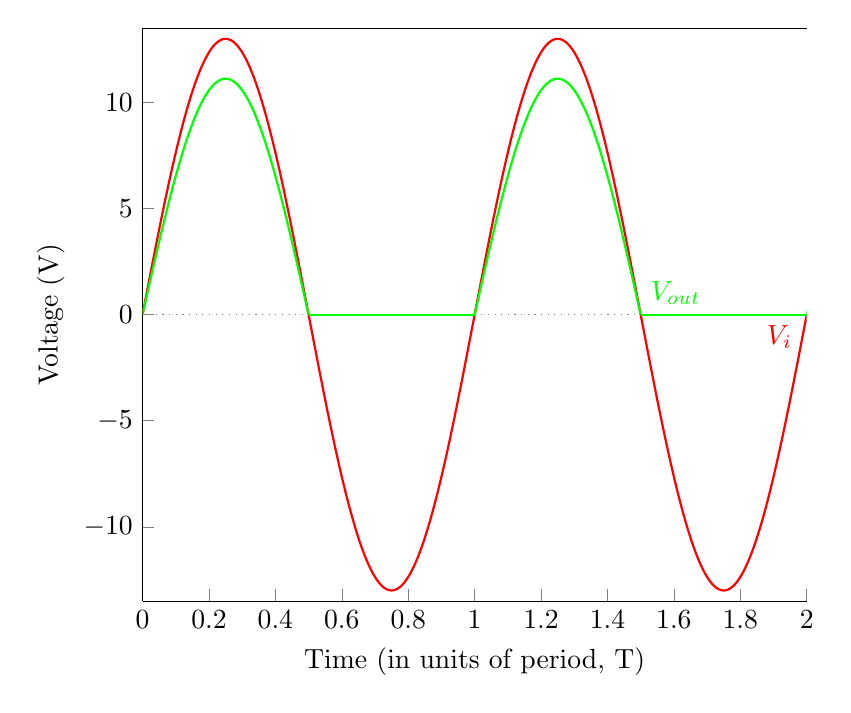
\begin{tikzpicture}[scale = 1]
        \pgfplotsset{
          scale only axis,
          xmin=0, xmax=2
        }
        \begin{axis}[
            axis y line*=left,
            ymin=-13.5, ymax=13.5,
            xlabel={Time (in units of period, T)},
            ylabel={Voltage ($\unit{\volt}$)},
            xtick pos=left,
            ytick pos=left
          ]
          
          \addplot[thick,red,samples=500,domain=0:2] (\x,{13*sin((2*pi*\x)*180/pi)}) node[pos=0.99, left]{$V_i$};
          \addplot[gray,dotted,samples=2,domain=0:2] (\x,{0});

          \addplot[thick,green,samples=500,domain=0:1/2] (\x,{11.12*sin((2*pi*\x)*180/pi)});
          \addplot[thick,green,samples=500,domain=1/2:1] (\x,{0});
          \addplot[thick,green,samples=500,domain=1:1.5] (\x,{11.12*sin((2*pi*\x)*180/pi)}) node[above right]{$V_{out}$};
          \addplot[thick,green,samples=500,domain=1.5:2] (\x,{0});
          \addplot[thick,green,samples=500,domain=2:2.5] (\x,{11.12*sin((2*pi*\x)*180/pi)});
        \end{axis}
      \end{tikzpicture}
    \end{center}
  \end{soln}
\end{document}